\section{Versuchsziel}
Die Bestimmung der Wellenlänge des Lichts das von einem Helium-Neon-Laser ausgesendet wird
sowie die Bestimmung des Brechungsindex von Luft und $\symup{CO}^2$  mit dem Michelson-Interferometers.
\section{Theorie}
\label{sec:Theorie}
Das Michelson-Interferometer nutzt, wie der Name bereits sagt, den Effekt der \textit{Interferenz}. Dieser Effekt tritt bei allen Wellen auf und beschreibt die Charakteristik der Überlagerung von Wellen. Bei besagter Überlagerung addieren sich die lokalen Auslenkungen (deren Betrag die \textit{Intensität} der Welle angibt) beider Wellen, weshalb sie sich gerade dann vollständig auslöschen (vorrausgesetzt sie besitzen die gleiche Amplitude), wenn ein Maximum und ein Minimum zusammentreffen. Interferenz ist also abhängig von der Phase des einfallenden Lichtes. Beim Michelson-Interferometer wird dieser Effekt erzeugt, indem ein Lichtstrahl geteilt wird und beide Teilstrahlen unterschiedlich lange Strecken zurücklegen, bevor sie wieder überlagert werden. Allerdings muss hierbei darauf geachtet werden, kohärentes Licht zu verwenden, d.h. eine Lichtquelle zu wählen, welche über einen möglichst langen Zeitraum gleichphasiges Licht emittiert, wie z.B. einen Laser. Ist dies Nicht gegeben, so liegt nicht nur ein Weglängen abhängiger Phasenunterschied vor, sondern auchnoch ein Phasenunterschied durch den zeitlichen Abstand der Ausstrahlung beider Quellen. Dieser Phasenunterschied ist scheinbar willkürlich und kann somit nicht aus den Messwerten harrausgerechnet werden.

Grundesetzlich funktioniert das Michelson-Interfereometer, wie in Darstellung
\ref{fig:SA} gezeigt, indem ein punktförmiger Lichtstrahl auf eine semipermeable
Platte (in der Darstellung P) geschossen wird. Dort wird dieser in zwei weitere
Strahlen geteilt die jeweils auf die Spiegel S1 und S2 treffen und dort reflektiert
werden. Bei erneutem treffen der Platte wird ein Teil der Strähle reflektiert
bzw. translatiert. Beide Strahlen interferieren wenn sie kohärend zu einander sind
und treffen auf den Detektor. Werden nun die Spiegel verschoben dann verändert sich
der Gangunterschied beider Straheln und der Detektor misst verschiedene Intensitäten.

\begin{figure}
  \centering
  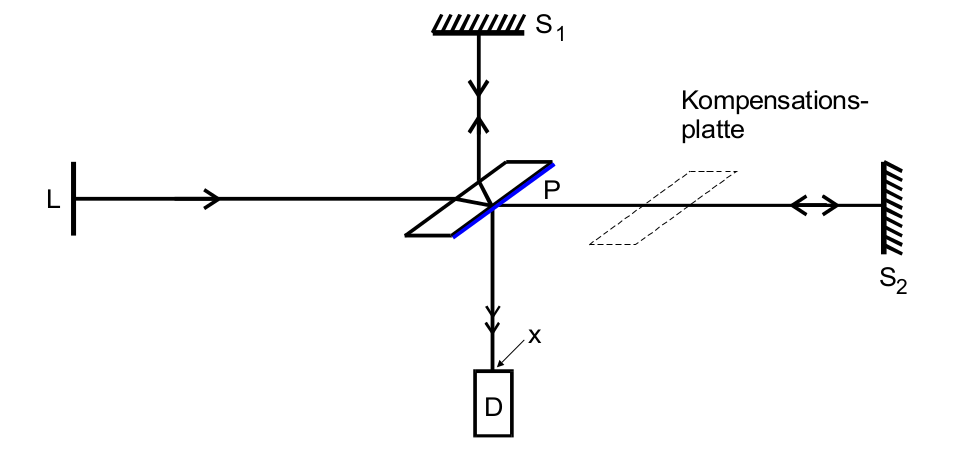
\includegraphics[height=5cm]{logos/SchemaInterf.png}
  \caption{Schematischer Aufbau des Michelson-Interferometers \cite{Anleitung}.}
  \label{fig:SA}
\end{figure}

Wird nun der Spiegel um $\Delta d$ verschoben so zählt der Detektor die autrettenden
Intensitätsmaxima. Daraus kann dann mit der Formel \cite{Anleitung}
\begin {equation}
  \Delta d = z \cdot \frac{\lambda}{2}
  \label{eqn:dd}
\end{equation}
die Wellenlänge $\lambda$ brechnet werden, dabei bezweichnet $z$ die Anzahl der
Interferenzmaxima. \\
Ist nun die Wellenlänge bekannt und der Lichtstrahl durch läuft ein Weg mit der
Länge $b$ durch ein Medium mit einem zusätzlichen Brechungsindex $ n + \Delta n$,
dann verändert sich auch der Wegunterschied der beiden interferierenden Strahlen.
Dieser beträgt nun genau $\Delta n \cdot b$. Diesen Wegunterschied wird nun
vergrößert in dem der Gasdruck in der Messzelle die die Strahlen passieren erhöht
wird (siehe Darstellung \ref{fig:KA}). Nun folgt für den Wegunterschied
\begin{equation}
  b \cdot \Delta n = z \frac{\lambda}{2}\;.
  \label{eqn:n}
\end{equation}
So kann nun der Brechungsindex $\Delta n$ bestimmt werden.
